\chapter{Gaussian Process Models on Multi-dimensional Grids}
\label{chap:gp_on_grids}


% \todo{Move this part to the intro and background. From here}

% Gaussian Processes (GP) have become a popular tool for regression which has lots of applications
% in engineering problems \citep{rasmussen2006gaussian}.
% They combine flexibility by allowing to approximate a wide range of smooth functions
% with simple structure of Bayesian inference and interpretable hyperparameters.

% GP regression algorithm has $\mathcal{O}(N^3)$ time complexity and $\mathcal{O}(N^2)$
% memory complexity, where $N$ is the size of the training sample.
% For large training sets (ten thousands or more) construction of GP regression becomes an intractable
% problem on current hardware.
Let us consider the case when the training set has a special structure
called {\em factorial Design of Experiments} (DoE) \citep{Montgomery2006DAE}.
In this structure, all the input variables are grouped into several {\em factors},
and the training set consists of the Cartesian product of the factors.
Such experimental designs arise naturally in many applications, especially in engineering.
Imagine we want to model some aerodynamic characteristic of an airfoil depending
on the shape of the airfoil and external conditions, like Mach number and angle of attack.
There are two ways to do it.
The first one is conducting computational fluid dynamic simulation to estimate
the desired characteristics.
Another way is building an airfoil and conducting wind tunnel experiments.
In the latter case, though it is expensive to build airfoils, it is easy to change the external
conditions so that we can select the external parameters on a regular grid
for each airfoil.
As a result, we have two sets of parameters.
One set describes the geometry of the airfoil, the other one - external conditions.
And in our measurements, those parameters have the Cartesian product structure.
In some cases, we can have missing values in such designs of the experiments.
It can either be some errors in measurements, computationally unstable procedures,
or just decrease the data set size.
In this case, we have {\em incomplete factorial Design of Experiments}.

The problem with such designs is that the training set size grows exponentially
with the number of factors.
The complexity of standard GP models does not allow to work with such training sets.
There are several methods for large-scale GP modeling; although they are not exact
and approximate, either the kernel function or the output of the GP model itself.
These approaches are general and can be applied to any data set.
More details can be found in Chapter~\ref{chap:unstructured_datasets}.

However, in case of full or incomplete factorial DoE, the special structure
of the data set can be exploited to derive computationally efficient
and the exact inference procedure.
There aren't many regression methods that consider the design of experiments.
There are several methods based on splines, which consider this special structure of the given data \citep{stone97polynomialsplines}.
A disadvantage of these methods is that they work only with one-dimensional factors
and cannot be applied to a more general case when the factors are multidimensional.
Another shortcoming is that such approaches do not have approximation accuracy evaluation procedure.
The missing values cannot be handled as well.


There is another problem that we are likely to encounter.
Factor sizes can vary significantly.
Engineers usually use large factors sizes if the corresponding input variables have a significant impact on function values.
Otherwise, the factors sizes are likely to be small,
i.e., the factor sizes are often selected using the knowledge from a subject domain \citep{rendall2008aircraftSurface}.
For example, if it is known that dependency on some variable is quadratic,
then the size of this factor will be three, as a larger size is redundant.
The difference between factor sizes can lead to the degeneracy of the GP model.
We will refer to this property of data set as {\em anisotropy}.

In this chapter, we develop an approach for fast, exact inference of the GP regression
model by considering
the factorial nature of the design of experiments in a general case of multidimensional factors.
Both full factorial and incomplete factorial designs are covered.
We also discuss how to choose the initial values of parameters for
the GP model and regularization in order to
consider possible anisotropy of the training data set.

The paper \citep{wilson2014fast} considers the same problem statement.
To efficiently train and evaluate a GP model, one needs a fast procedure
to calculate $\mathbf{K}^{-1}\mathbf{y}$,
where $\mathbf{K}$ is a kernel matrix,
and an efficient procedure to evaluate the determinant of the kernel matrix.
The authors of \citep{wilson2014fast} exploit the structure in the data set
to efficiently calculate both components in the case of full factorial design of experiments.
In the case of incomplete factorial design of experiments,
they apply the preconditioned conjugate gradient (PCG) method to calculate $\mathbf{K}^{-1}\mathbf{y}$.
It is based on an efficient approach for the matrix-vector product $\mathbf{K}\mathbf{y}$,
which, however, gives an exact answer only in the limit when the parameter of the method goes to infinity.
Empirically, the PCG in this case requires a small number of iterations (much smaller than the dataset size).
In contrast, this chapter of the dissertation shows an approach that calculates
$\mathbf{K}^{-1}\mathbf{y}$ in case of incomplete factorial deign of experiments exactly.
We also derive the exact number of iterations required for conjugate gradients approach to converge.
We show that the method is efficient when the number of missing points is small or very large.
Another difference is that we calculate the determinant of the kernel matrix exactly but in about
$\mathcal{O}(N^2)$ operations, whereas \citep{wilson2014fast} make an approximation to the determinant
but in $\mathcal{O}(N)$ iterations.
We also introduce a special regularization that allows to reduce degeneration effect.



The main contributions of this chapter are as follows
\begin{itemize}
  \item We develop a computationally efficient approach for the case of the multi-dimensional
  data set.
  \item For the case of multi-dimensional grid with missing points, we derive a conjugate gradient-based approach for matrix inversion, which provably converges in $\mathcal{O}(\min (R, N))$
  iterations, where $R$ is the number of missing points.
  \item We propose a special regularization for the data sets on multi-dimensional grids
  that makes the GP model less prone to degeneration.
\end{itemize}

% In this chapter we consider the data sets with special structure.
% We suppose that input variables are grouped into several sets and
% input points form the Cartesian product of the sets.
% Such designs of the experiment are called {\em factorial design of experiments} (DoE) and
% common in many engineering problems \citep{Montgomery2006DAE}.
% The sets of groups of variables are called {\em factors}.
% The number of different values in a factor is called {\em factor size}.

% When the factorial DoE is used the size of the data set can be very large
% as it grows exponentially with the dimension of input variables.
% We also consider problems where some points are missing from the
% Cartesian product.
% However, in both cases, an efficient algorithm can be constructed
% by considering the structure of the dataset.


\section{Factorial design of experiments}
Let us refer to sets of points
${\omega_k = \{ x_{i_k}^k \in {\rm X}_k \}_{i_k = 1}^{n_k}}$,
${\rm X}_k \subset \mathbb{R}^{d_k}, \, k = \overline{1, K}$ as {\em factors}.
A set of points $\Omega$ is referred to as a factorial design of experiments
if it is a Cartesian product of factors
\begin{equation}
  \label{eq:factorial_design}
    \Omega = \omega_1 \times \omega_2 \times \cdots \times \omega_k =
    \{ [x_{i_1}^1, \ldots, x_{i_K}^K], \{ i_k = 1, \ldots, n_k\}_{k = 1}^K \}.
\end{equation}
The elements of $\Omega$ are vectors of a dimension $d = \sum_{i = 1}^K d_i$ and
the sample size is a product of sizes of all factors $N = \prod_{i = 1}^K n_i$.
If all the factors are one-dimensional, $\Omega$ is a full factorial design.
But in a more general case, factors are multidimensional (see example in Figure \ref{fig:multidim_factor}).

\begin{figure}
  \centering
  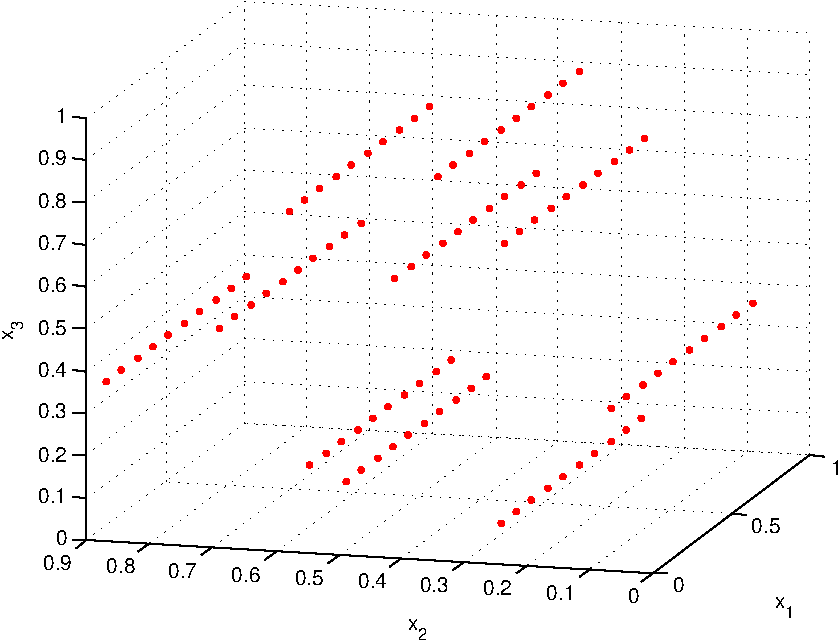
\includegraphics[width=0.5\textwidth]{figures/gp_on_grid/multidim_factor.pdf}
  \caption{Example of a multidimensional factor. In the figure, $x_1$ is a usual one-dimensional factor
  and $(x_2, x_3)$ is a two-dimensional factor.}
  \label{fig:multidim_factor}
\end{figure}


\section{Tensor and related operations}
Let us introduce tensor notation and some related operations that will be used
later.

A {\em tensor} $\mathcal{Y}$ is a $K$-dimensional matrix of size $n_1 \times n_2 \times \cdots \times n_K$
\citep{kolda09tensordecompositions}:
\begin{equation}
  \label{eq:tensor}
  \mathcal{Y} = \{ y_{i_1, i_2, \ldots, i_K}, \{i_k = 1, \ldots, n_k \}_{k = 1}^K \}.
\end{equation}

By $\mathcal{Y}^{(j)}$, we will denote a matrix consisting of elements of the tensor $\mathcal{Y}$
whose rows are $1 \times n_j$ slices of $\mathcal{Y}$ with fixed indices
$i_{j + 1}, \ldots, i_K, i_1, \ldots, i_{j - 1}$ and altering index $i_j = 1, \ldots, n_j$.
In case of a $2$-dimensional tensor, it holds that
${\mathcal{Y}^{(1)} = \mathcal{Y}^T}$ and $\mathcal{Y}^{(2)} = \mathcal{Y}$.

Now let us introduce the multiplication of a tensor by a matrix along the direction $i$.
Let $B$ be some matrix of size $n_i \times n_i'$.
Then the product of the tensor $\mathcal{Y}$ and the matrix $B$ along the direction $i$
is a tensor $\mathcal{Z}$ of size $n_1 \times \cdots \times n_{i - 1} \times n_i' \times n_{i + 1} \times \cdots \times n_K$
such that $\mathcal{Z}^{(i)} = \mathcal{Y}^{(i)}B$.
We will denote this operation by $\mathcal{Z} = \mathcal{Y} \otimes_i B$.
For a $2$-dimensional tensor $\mathcal{Y}$, multiplication along the first direction is a left multiplication
by matrix $\mathcal{Y} \otimes_1 B = B^T \mathcal{Y}$,
and along the second direction --- is a right multiplication $\mathcal{Y} \otimes_2 B = \mathcal{Y} B$.

Multiplication of a tensor by a matrix along some direction is closely related to the Kronecker product.
Let's consider an operation {\em vec}, which, for every multidimensional matrix $\mathcal{Y}$
returns a vector containing all elements of $\mathcal{Y}$.
An inner product of tensors $\mathcal{Y}$ and $\mathcal{Z}$ is the inner product of vectors
${\rm vec}(\mathcal{Y})$ and ${\rm vec}(\mathcal{Z})$
\[
\left < \mathcal{Y}, \mathcal{Z}\right > = \left < {\rm vec}(\mathcal{Y}), {\rm vec}(\mathcal{Z}) \right >.
\]

For every multidimensional matrix $\mathcal{Y}$ of size $n_1 \times n_2 \times \cdots \times n_K$
and $n_i \times p_i$ size matrices $B_i$, $i = 1, \ldots, K$ the following identity holds \citep{loan2000kronecker}
\begin{equation}
  \label{eq:kronecker_product}
    (B_1 \otimes B_2 \cdots \otimes B_K) {\rm vec}(\mathcal{Y}) =
    {\rm vec} (\mathcal{Y} \otimes_1 B_1^T \cdots \otimes_K B_K^T),
\end{equation}
where symbol $\otimes$ denotes the Kronecker product.

Let's compare the complexity of the right and the left hand sides of (\ref{eq:kronecker_product}).
For simplicity, we assume that all the matrices $B_i$ are quadratic of size $n_i \times n_i$ and
$N = \prod n_i$.
Then computation of the left-hand side of (\ref{eq:kronecker_product}) requires
$N^2$ operations (of additions and multiplications) not considering the complexity of the Kronecker product
while the right hand side requires $N \sum_i n_i$ operations.


\subsection{Efficient log-likelihood calculation}
\label{sec:calc_loglikelihood}
Now, let us see how the introduced operations can be used for efficient
computation of the predictive distribution and the marginal log-likelihood.

Covariance function (\ref{eq:covariance_function}) can be represented as
a product of covariance functions each depending only on the variables from one factor
\begin{equation}
  \label{eq:covariance_function_general}
  k(\mathbf{x}_p, \mathbf{x}_q) = \prod_{i = 1}^K k_i(x_p^i, x_q^i),
\end{equation}
where $x_p^i, x_q^i \in \mathbb{R}^{d_i}$ belong to the same factor $\omega_i$.
For the squared exponential function, we have $k_i(x_p^i, x_q^i) = \omega_{f, i}^2\exp \left ( -\sum_j^{d_i} \left (\theta_i^{(j)} \right )^2
  \big (x_p^{(j), i} - x_q^{(j), i} \big )^2 \right )$,
where $x_p^{(j), i}$ is a $j$-th component of $x_p^i$.
Note that in general case covariance functions $k_i$ are not necessarily squared exponential, they can be of different types for different factors.
It allows to consider the special features of factors (knowledge from a subject domain) if they are known.
In such a case, the function defined by (\ref{eq:covariance_function_general}) is still a valid
covariance function being the product of separate covariance functions.
From now on, we will denote by $\theta_i = (\theta_i^{(1)}, \ldots, \theta_i^{(d_i)})$ the set of hyperparameters for covariance
function of the $i$-th factor and let $\boldsymbol{\theta} = (\theta_1, \ldots, \theta_K)$.

Such form of the covariance function and the factorial DoE
allows us to represent the covariance matrix as the Kronecker product
\begin{equation}
  \label{eq:covariance_kronecker}
  \mathbf{K}_f = \bigotimes_{i = 1}^K\mathbf{K}_i,
\end{equation}
where $\mathbf{K}_i$ is a covariance matrix defined by the $k_i$ covariance function
computed at points from the $i$-th factor $\omega_i$.

The Kronecker product of matrices can be efficiently inverted due to the following
property
\[
(A \otimes B)^{-1} = A^{-1} \otimes B^{-1}
\]
if $A$ and $B$ are invertible matrices.
If $A$ has size $n_a \times n_a$ and $B$ has size $n_b \times n_b$ then
the left side of the above equation requires $\mathcal{O}(n_a^3n_b^3)$ operations
while the right hand side requires only $\mathcal{O}(n_a^3 + n_b^3)$ operations
and this is much less.
However, we have to invert the matrix $\mathbf{K}_y = \mathbf{K}_f + \sigma_{noise}^2 \mathbf{I}$.
For this, we use the Singular Value Decomposition (SVD)
\[
\mathbf{K}_i = \mathbf{U}_i \mathbf{D}_i \mathbf{U}_i^T,
\]
where $\mathbf{U}_i$ is an orthogonal matrix of eigenvectors of matrix $\mathbf{K}_i$
and $\mathbf{D}_i$ is a diagonal matrix of eigenvalues.
Using the properties of the Kronecker product and representing an identity matrix as
$\mathbf{I}_{d_i} = \mathbf{U}_i \mathbf{U}_i^T$ we obtain
\begin{equation}
  \label{eq:inverse_covariance}
  \mathbf{K}_y^{-1} = \left (\bigotimes_{i = 1}^K \mathbf{U}_i \right ) \left (
    \left [\bigotimes_{i = 1}^K \mathbf{D}_i \right ] + \sigma_{noise}^2 \mathbf{I} \right )^{-1}
  \left ( \bigotimes_{i = 1}^K \mathbf{U}_i^T \right ).
\end{equation}

Computing SVD for all $\mathbf{K}_i$ requires $\mathcal{O}(\sum_k n_k^3)$ operations.
Calculation of the Kronecker product in (\ref{eq:inverse_covariance}) has complexity $\mathcal{O}(N^2)$.
So, this gives us overall complexity $\mathcal{O}(N^2)$ for calculation of expressions for the log-likelihood,
the predictive mean, and the covariance.
It is faster than the straightforward calculations; however, it can be improved.

Equations~\eqref{eq:gp_posterior} and \eqref{eq:loglikelihood}
for GP regression do not require explicit inversion of $\mathbf{K}_y$.
In each equation, it is multiplied by vector $\mathbf{y}$ (or $\mathbf{k}_*$).
So, we will compute $\mathbf{K}_y^{-1} \mathbf{y}$ instead of explicitly inverting
$\mathbf{K}_y$ and then multiplying it by the vector $\mathbf{y}$.

Let $\mathcal{Y}$ be a tensor containing values of the vector $\mathbf{y}$ such that
${\rm vec}(\mathcal{Y}) = \mathbf{y}$.
Now using identities (\ref{eq:kronecker_product}) and (\ref{eq:inverse_covariance})
we can write $\mathbf{K}_y^{-1}\mathbf{y}$ as
\begin{align}
  \label{eq:fast_inverse_covariance}
    \mathbf{K}_y^{-1}\mathbf{y} &= \left ( \bigotimes_{i = 1}^K \mathbf{U}_i \right )
    \left ( \left [\bigotimes_{i = 1}^K \mathbf{D}_i \right ] + \sigma_{noise}^2 \mathbf{I} \right )^{-1} \times
    {\rm vec}(\mathcal{Y} \otimes_1 \mathbf{U}_1 \cdots \otimes_K \mathbf{U}_K) = \nonumber \\
    &= {\rm vec}\left [ \left ((\mathcal{Y} \otimes_1 \mathbf{U}_1 \cdots \otimes_K \mathbf{U}_K) * \mathcal{D}^{-1} \right ) \otimes_1
    \mathbf{U}_1^T \cdots \otimes_K \mathbf{U}_K^T \right ],
\end{align}
where $\mathcal{D}$ is a tensor constructed by transforming the diagonal of matrix
$\big [\bigotimes_k \mathbf{D}_k \big ] + \sigma_{noise}^2 \mathbf{I}$ into a tensor.

The elements of the tensor $\mathcal{D}$ are eigenvalues of the matrix $\mathbf{K}_y$,
therefore, its determinant can be calculated as
\begin{equation}
  \label{eq:fast_determinant}
  |\mathbf{K}_y| = \prod_{i_1, \ldots, i_K} \mathcal{D}_{i_1, \ldots, i_K}.
\end{equation}

\begin{proposition}
  The computational complexity of the log likelihood (\ref{eq:loglikelihood}), where $\mathbf{K}_y^{-1}y$ and
  $|\mathbf{K}_y|$ are calculated using (\ref{eq:fast_inverse_covariance}) and (\ref{eq:fast_determinant}), is
  \begin{equation}
    \mathcal{O} \left (\sum_{i = 1}^K n_i^3 + N\sum_{i = 1}^K n_i \right ).
  \end{equation}
\end{proposition}
\begin{proof}
  Let's calculate the complexity of computing $\mathbf{K}_y^{-1} \mathbf{y}$ using (\ref{eq:fast_inverse_covariance}).
  Computation of the matrices $\mathbf{U}_i$ and $\mathbf{D}_i$ requires $\mathcal{O}(\sum_i n_i^3)$ operations.
  Multiplication of the tensor $\mathcal{Y}$ by the matrices $\mathbf{U}_i$ requires $\mathcal{O}(N\sum_i n_i)$ operations.
  Further, a component-wise product of the obtained tensor and the tensor $\mathcal{D}^{-1}$ requires $\mathcal{O}(N)$
  operations.
  And the complexity of multiplication of the result by the matrices $\mathbf{U}_i$ is again $\mathcal{O}(N\sum_i n_i)$.
  The determinant, calculated by equation (\ref{eq:fast_determinant}), requires $\mathcal{O}(N)$ operations.
  Thus, the overall complexity of computing (\ref{eq:fast_inverse_covariance}) is
  ${\mathcal{O}(\sum_{i = 1}^K n_i^3 + N\sum_{i = 1}^K n_i)}$.
\end{proof}

For more illustrative estimate of the computational complexity,
suppose that $n_i \ll N$ (number of factors is large and their sizes are close).
In this case, it holds that
$\mathcal{O}(N\sum_i n_i) = \mathcal{O}(N^{1 + \frac{1}{K}})$ and this is
much less than $\mathcal{O}(N^3)$.

To optimize the log-likelihood over the hyperparameters, we use a gradient-based method.
The derivatives of the log likelihood with respect to the hyperparameters take the form
\begin{equation}
\label{eq:loglikelihood_derivative}
    \frac{\partial}{\partial \theta} \left (\log \vphantom{p(\mathbf{y} | \mathbf{X}, \sigma_f, \sigma_{noise})}
    p(\mathbf{y} | \mathbf{X}, \sigma_f, \sigma_{noise}) \right ) =
    -\frac12 {\rm Tr}(\mathbf{K}_y^{-1} \mathbf{K}') + \frac12\mathbf{y}^T \mathbf{K}_y^{-1} \mathbf{K}' \mathbf{K}_y^{-1} \mathbf{y},
\end{equation}
where $\theta$ is one of the hyperparameters $\theta_i$, $\sigma_{noise}$ or $\omega_{f, i}, i = 1, \ldots, d$ and
$\mathbf{K}' = \dfrac{\partial \mathbf{K}}{\partial \theta}$.
$\mathbf{K}'$ is also the Kronecker product
\[
\mathbf{K}' = \mathbf{K}_1 \otimes \cdots \otimes \mathbf{K}_{i - 1} \otimes \frac{\partial \mathbf{K}_i}{\partial \theta}
\otimes \mathbf{K}_{i + 1} \otimes \cdots \otimes \mathbf{K}_K,
\]
where $\theta$ is a parameter of the $i$-th covariance function.
Denoting by $\mathcal{A}$, a tensor such that ${\rm vec}(\mathcal{A}) = \mathbf{K}_y^{-1}\mathbf{y}$
the second term in equation (\ref{eq:loglikelihood_derivative}) can be efficiently computed
using the same technique as in (\ref{eq:fast_inverse_covariance}):
\begin{align}
  \label{eq:fast_derivative_second_term}
    \frac12\mathbf{y}^T \mathbf{K}_y^{-1} \mathbf{K}'\mathbf{K}_y^{-1} \mathbf{y} =
    \left < \mathcal{A}, \mathcal{A}
    \vphantom{\frac{\partial \mathbf{K}_i^T}{\partial \theta}}
    \right .
    & \otimes_1 \mathbf{K}_1^T \otimes_2 \cdots \otimes_{i - 1}
    \mathbf{K}_{i - 1}^T \otimes_i
    \frac{\partial \mathbf{K}_i^T}{\partial \theta} \otimes_{i + 1} \nonumber \\
    &\left .
    \vphantom{\frac{\partial \mathbf{K}_i^T}{\partial \theta}}
    \otimes_{i + 1} \mathbf{K}_{i + 1}^T \otimes_{i + 2} \cdots \otimes_K \mathbf{K}_K^T \right >.
\end{align}
The complexity of calculating this term of derivative is the same as the complexity of
equation (\ref{eq:fast_inverse_covariance}).

Now, let us compute the first term
\begin{equation}
  \begin{split}
    {\rm Tr}(\mathbf{K}_y^{-1} \mathbf{K}') = &\; {\rm Tr} \left (
      \left (\bigotimes_{i = 1}^K \mathbf{U}_i \right ) \mathbf{D}^{-1} \left (\bigotimes_{i = 1}^K \mathbf{U}_i^T \right ) \mathbf{K}'
    \right)= \\
    = &\; {\rm Tr} \left (\mathbf{D}^{-1} \left (\bigotimes_{i = 1}^K \mathbf{U}_i^T \mathbf{K}_i' \mathbf{U}_i \right ) \right ) = \\
    = &\; \left < {\rm diag} \left (\mathbf{D}^{-1} \right ), {\rm diag} \left (\bigotimes_{i = 1}^K \mathbf{U}_i \mathbf{K}_i' \mathbf{U}_i \right ) \right > = \\
    = &\; \left < {\rm diag} \left (\mathbf{D}^{-1} \right ),  \bigotimes_{i = 1}^K {\rm diag} \left ( \mathbf{U}_i \mathbf{K}_i' \mathbf{U}_i \right ) \right >,
  \end{split}
\end{equation}
where ${\rm diag}\big(A \big)$ is a vector of diagonal elements of a matrix $A$,
$\; \mathbf{D} = \bigotimes_i \mathbf{D}_i + \sigma_{noise}^2 \mathbf{I}$.


The computational complexity of this derivative term is the same as the computational
complexity of equation (\ref{eq:fast_derivative_second_term}).

Thus, we obtain
\begin{proposition}
  The computational complexity of calculating derivatives of the log likelihood is
  ${\mathcal{O}\left (\sum\limits_{i = 1}^K n_i^3 + N \sum\limits_{i = 1}^K n_i \right )}$.
\end{proposition}

\begin{table}[t]
  \caption{Runtime (in seconds) of tensored GP and original GP algorithms.}
  \label{tb:runtime}
  \vskip 0.15in
  \begin{center}
    \begin{small}
      \begin{sc}
        \begin{tabular}{rrr}
          \hline
          %\abovespace\belowspace
          & original GP   & tensored GP \\
          64     & 0.8    & 0.16 \\
          160    & 2.69   & 0.16 \\
          432    & 14.31  & 0.74 \\
          1000   & 120.38 & 1.02 \\
          2000   & 970.21 & 1.11 \\
          10240  & ---    & 33.18 \\
          64000  & ---    & 74.9 \\
          160000 & ---    & 175.15 \\
          400000 & ---    & 480.14\\
          \hline
          %\abovespace\belowspace
        \end{tabular}
      \end{sc}
    \end{small}
  \end{center}
  \vskip -0.1in
\end{table}

Table \ref{tb:runtime} contains training times for
original GP and proposed GP regression for different sample sizes.
The experiments were conducted on a PC with Intel i7 2.8 GHz processor and
4 GB RAM.
For the original GP, we used GPML Matlab code \citep{gpmltoolbox}.
We also adopted the GPML code to use tensor operations.
The results illustrate that the proposed approach is much faster than the original GP
and allows making approximations using extremely large data sets.

\subsection{Anisotropy}
In this section, we will consider an anisotropy problem.
As it was mentioned in an engineering practice, factorial designs are
often anisotropic, i.e., the sizes of factors differ significantly.
It is a common case for the GP regression to become degenerate in such a situation.
Suppose the given DoE consists of two one-dimensional factors
with sizes $n_1$ and $n_2$.
Assume that $n_1 \ll n_2$.
Then one could expect the length-scale for the first factor to be much greater than
the length-scale for the second factor (or $\theta_1 \ll \theta_2$).
However, in practice, we often observe the opposite $\theta_1 \gg \theta_2$.
This happens because the optimization algorithm stacks in a local maximum during maximization over
the hyperparameters as the objective function (the log-likelihood) is non-convex with lots of local maxima.
We get an undesired effect of degeneracy:
in the region without training points, the approximation is constant, and it has sharp peaks at training points.
This situation is illustrated in Figure \ref{fig:anisotropy_degeneracy}
(compare with the true function in Figure \ref{fig:anisotropy_degeneracy_true}).

Let us denote length-scales as $l_k^{(i)} = \big [\theta_k^{(i)} \big ]^{-1}$.
To incorporate our prior knowledge about factor sizes into regression model
we introduce prior distribution on the hyperparameters~$\boldsymbol{\theta}$:
\begin{equation}
  \label{eq:prior}
  \frac{\theta_k^{(i)} - a_k^{(i)}}{b_k^{(i)} - a_k^{(i)}} \sim \mathcal{B}e(\alpha, \beta), \, \{ i = 1, \ldots, d_k\}_{k = 1}^K,
\end{equation}
i.e., prior on hyperparameter $\theta_k^{(i)}$ is a beta distribution with parameters $\alpha$
and $\beta$ scaled to some interval $\left [a_k^{(i)}, b_k^{(i)} \right ]$.

The log likelihood then has the form
\begin{equation}
  \label{eq:loglikelihood_prior}
  \begin{split}
    \log p(\mathbf{y} \, | \, \mathbf{X}, \boldsymbol{\theta}, \sigma_f, \sigma_{noise}) = -& \frac12 \mathbf{y}^T \mathbf{K}_y^{-1}\mathbf{y} - \frac12 \log |\mathbf{K}_y| - \\
    - \frac{N}{2} \log 2 \pi + & \sum_{k, i} \left ( (\alpha - 1) \log(\theta_k^{(i)}) + \right . \\
    + (\beta - 1) \log (1 - &  \left . \theta_k^{(i)})  \right ) - d \log({\rm B}(\alpha, \beta)),
  \end{split}
\end{equation}
where ${\rm B}(\alpha, \beta)$ is a beta function.

By introducing such prior, we restrict parameters $\theta_k^{(i)}$ to belong
to some interval $\left [a_k^{(i)}, b_k^{(i)} \right ]$ (or length-scales $l_k^{(i)}$ to belong to the interval
$\left [\big (b_k^{(i)} \big)^{-1}, \big (a_k^{(i)} \big )^{-1} \right ]$).
It seems reasonable that for an approximation to fit the training points
the length-scale is not needed to be much less than the distance between points.
That's why we choose the lower bound for the length-scale $l_k^{(i)}$ to be $c_k * \min\limits_{x, y \in \omega_k, x^{(i)} \ne y^{(i)}} ||x^{(i)} - y^{(i)}||$
and the upper bound for the length-scale to be ${C_k * \max\limits_{x, y \in \omega_k} ||x^{(i)} - y^{(i)}||}$.
The value $c_k$ should be close to 1.
If it is too small, we are taking risks to overfit the data by allowing small length-scales.
If $c_k$ is too large, we will underfit the data by allowing only large length-scales and forbidding small ones.
Constants $C_k$ must be much greater than $c_k$ to permit large length-scales and preserve flexibility.
In this work, we used $c_k = 0.5$ and $C_k = 100$.
Such values of $c_k$ and $C_k$ worked rather well in our test cases.

Parameters of beta distribution was set to $\alpha = \beta = 2$ to get
symmetrical probability distribution function (see Figure \ref{fig:beta}) because
we do not know a priori if the values of GP parameters should be large or small.
The chosen prior distribution penalizes too large and too small values of parameters $\theta_k$
as they are undesirable.

Figure \ref{fig:nondegenerate_tensorGP} illustrates the approximation
of the GP regression with introduced prior distribution (and initialization described in Section \ref{sec:tensor_gp_init}).
The hyperparameters were chosen such that the approximation
is nondegenerate.

\begin{figure}
  \centering
  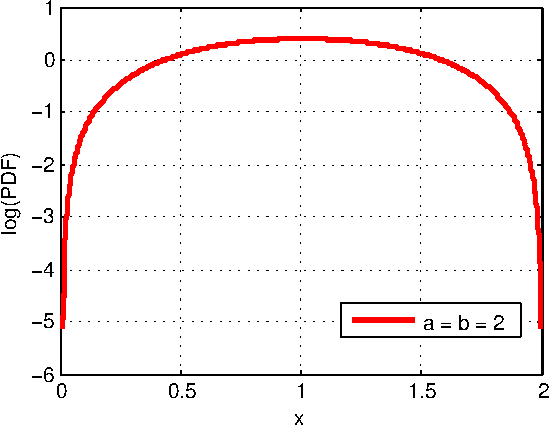
\includegraphics[width=0.3\textwidth]{figures/gp_on_grid/beta.pdf}
  \caption{Logarithm of Beta distribution probability density function, rescaled to $[0.01, 2]$ interval,
    with parameters $\alpha = \beta = 2$.}
  \label{fig:beta}
\end{figure}


\subsection{Initialization}
\label{sec:tensor_gp_init}
It is also important to choose reasonable initial values of hyperparameters
in order to converge to a good solution during parameter optimization.
The kernel-widths for different factors should have different scales because
corresponding factor sizes have different numbers of levels.
Hence, it seems reasonable to use the average distance between points in a factor as an initial value
\begin{equation}
  \label{eq:initialization}
  \theta_k^{(i)} = \left [ \frac{1}{n_k} \left ( \max\limits_{x \in \omega_k}(x^{(i)}) - \min\limits_{x \in \omega_k}(x^{(i)}) \right ) \right ]^{-1}.
\end{equation}
% i.e. the initial length-scale is an average distance between neighboring points in factor.

\begin{figure}
  \centering
  \begin{subfigure}[b]{0.45\textwidth}
      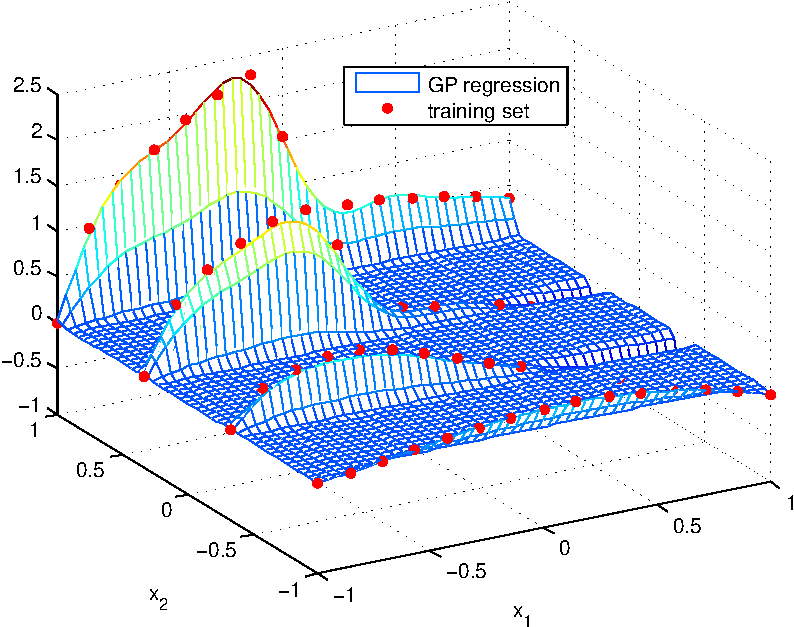
\includegraphics[width=\textwidth]{figures/gp_on_grid/degeneration.pdf}
      \caption{Degeneracy of the GP model in case of anisotropic data set.
        The length-scales for this model are $l_1 = 0.286, l_2 = 0.033$
        whereas factor sizes are $n_1 = 15, n_2 = 4$.}
      \label{fig:anisotropy_degeneracy}
  \end{subfigure}
  \begin{subfigure}[b]{0.45\textwidth}
      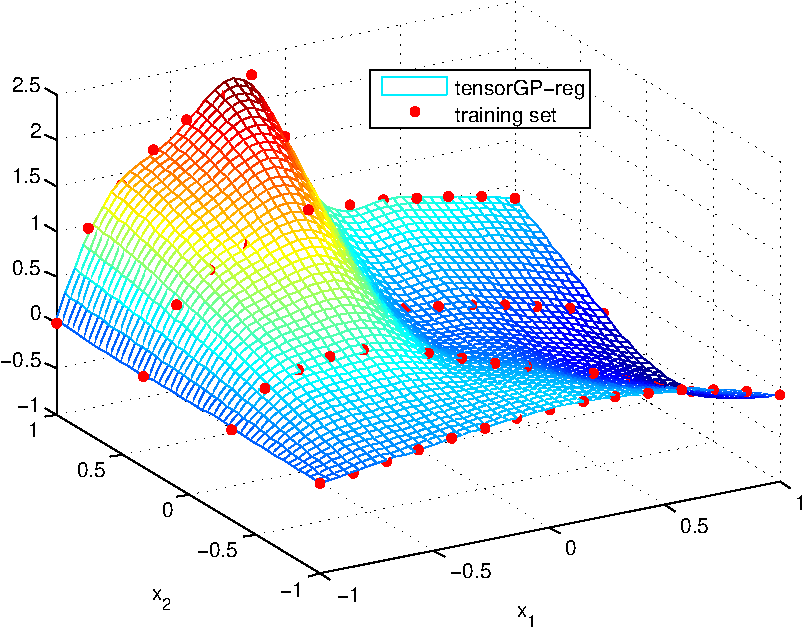
\includegraphics[width=\textwidth]{figures/gp_on_grid/nondegenerate_tensorGP.pdf}
      \caption{The GP regression with proposed prior distribution and initialization.}
      \label{fig:nondegenerate_tensorGP}
  \end{subfigure}
  \begin{subfigure}[b]{0.45\textwidth}
      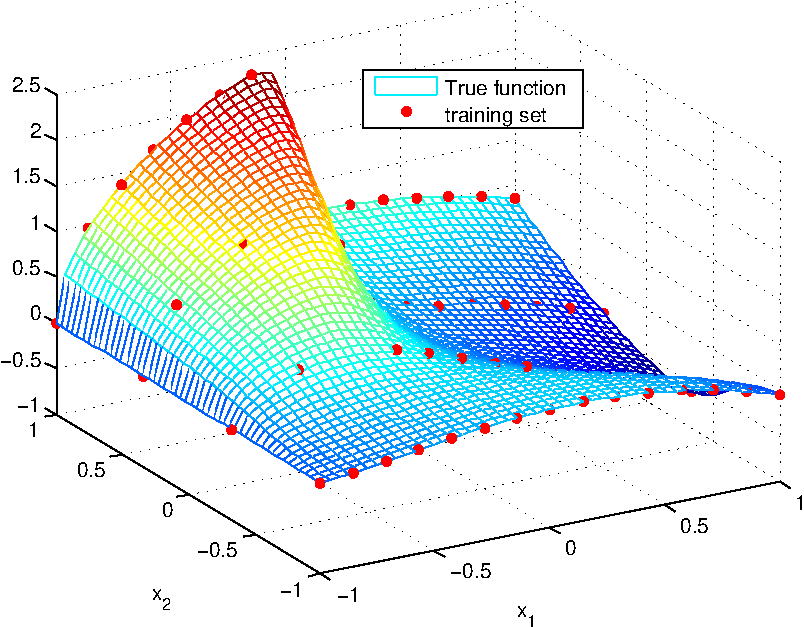
\includegraphics[width=\textwidth]{figures/gp_on_grid/degeneration_true.pdf}
      \caption{True function.}
      \label{fig:anisotropy_degeneracy_true}
  \end{subfigure}
\end{figure}


\section{Experiments}
The proposed algorithm was tested on a set of test functions \citep{lappeenranta, ETH}.
The functions have different input dimensions from 2 to 6 and the sample sizes $N$
varied from $100$ to about $200000$.
For each function, several factorial anisotropic training sets were generated.
We will test the following algorithms: GP with tensor computations (tensorGP),
GP with tensor computations and prior distribution (tensorGP-reg),
the sparse pseudo-point input GP (FITC) \citep{snelson06sparsegaussian}.
For the FITC method, we used GPML Matlab code \citep{gpmltoolbox}.
The number of inducing points of FITC algorithm varied from $M = 500$ for small samples (up to $5000$ points)
to $M = 70$ for large samples (about $10^5$ points) in order to obtain approximation in reasonable time
(complexity of FITC algorithm is $\mathcal{O}(M^2N)$).
For tensorGP and tensorGP-reg, we adopted GPML code to use tensor operations, proposed prior distribution
and initialization.

To assess the quality of approximation, a mean squared error was used
\begin{equation}
  \label{eq:mse}
  {\rm MSE} = \frac{1}{N_{test}} \sum_{i = 1}^{N_{test}} (\hat{f}(\mathbf{x}_i) - f(\mathbf{x}_i))^2.
\end{equation}

To compare different algorithms, Dolan-Mor\'{e} curves are used \citep{dolanMore}.
The idea of Dolan-Mor\'{e} curves is as follows.
Let $t_{p, a}$ be an error of an $a$-th algorithm on a $p$-th problem and $r_{p, a}$
be a performance ratio
\[
r_{p, a} = \frac{t_{p, a}} {\min\limits_s(t_{p, s})}.
\]
Then Dolan-Mor\'{e} curve is a graph of $\rho_a(\tau)$ function where
\[
\rho_a(\tau) = \frac{1}{n_p}{\rm size} \{p: r_{p, a} \le \tau \},
\]
which can be thought of as a probability for the  $a$-th algorithm to have performance
ratio within factor $\tau \in \mathbb{R}_+$.
The higher the curve $\rho_a(\tau)$ is located, the better the corresponding algorithm works.
$\rho_a(1)$ is the number of problems on which the $a$-th algorithm showed the best performance.

As expected, tensorGP performs better than FITC, as it uses all the information
contained in the training sample.
The introduced prior distribution is more suited for anisotropic data and hence,
GP with such prior (tensorGP-reg) performs even better (see Figure \ref{fig:dolan_more}).

To compare the run-time performances of the algorithms, we plotted Dolan-Mor{'e} curves
where instead of approximation error, the training time was used (see Figure \ref{fig:dolan_more_time}).
Here, we see that tensorGP and tensorGP-reg outperform FITC algorithm.

\begin{figure}
  \centering
  \begin{subfigure}[b]{0.45\textwidth}
      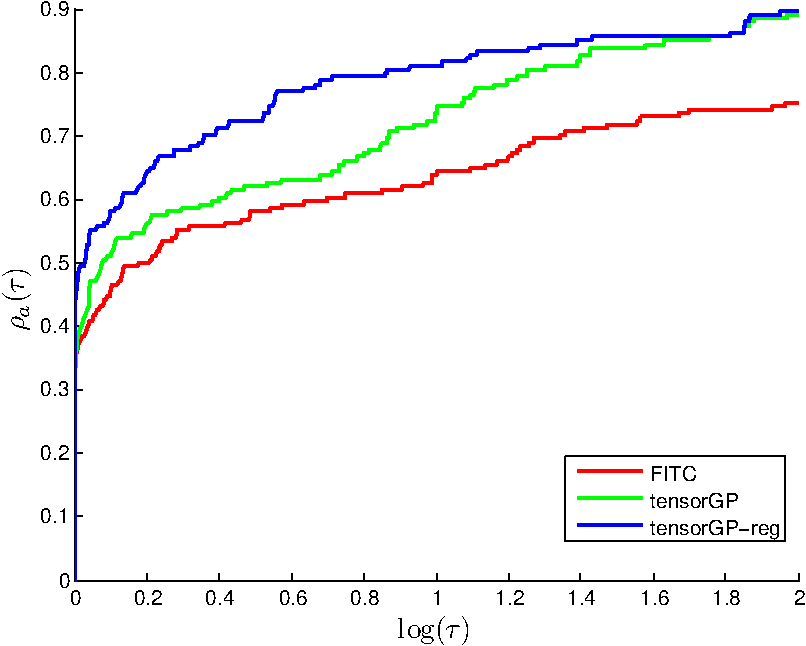
\includegraphics[width=\textwidth]{figures/gp_on_grid/dolan_more.pdf}
      \caption{Approximations accuracy.}
      \label{fig:dolan_more}
  \end{subfigure}
  \begin{subfigure}[b]{0.45\textwidth}
      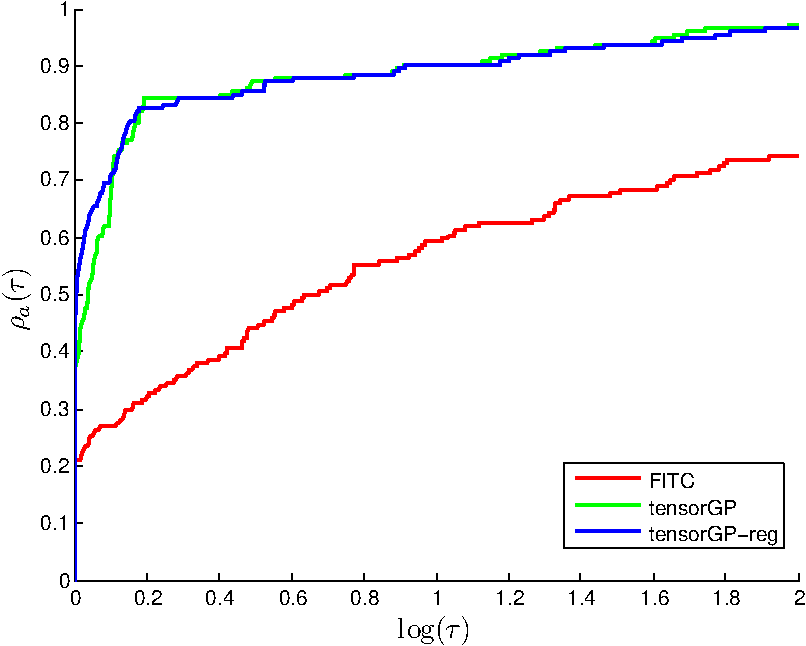
\includegraphics[width=\textwidth]{figures/gp_on_grid/dolan_more_time.pdf}
      \caption{Run-times.}
      \label{fig:dolan_more_time}
  \end{subfigure}
  \caption{Dolan-Mor\'e curves for tensorGP, tensorGP-reg and FITC algorithms
        in logarithmic scale.
        The higher the curve lies, the better the corresponding algorithm performs.}
\end{figure}

\subsection{Rotating disc problem}

In this section, we will consider a real-world problem of rotating disc shape design.
Such kind of problems often arise during aircraft engine design and in turbomachinery \citep{armand1995structural}.

In this problem, a disc of an impeller is considered.
It is rotated around the shaft.
The geometrical shape of the disc considered here is parameterized by 6 variables
$\mathbf{x} = (h_1, h_2, h_3, h_4, r_2, r_3)$ ($r_1$ and $r_4$ are fixed), see Figures \ref{fig:rotating_disc_parametrization} and \ref{fig:rotating_disc_objectives}.
The task of an engineer is to find such geometrical shape of the disc that minimizes the disc's weight and the contact pressure $p_1$ between
the disc and the shaft while constraining the maximum radial stress $Sr_{max}$ to be less than some threshold.
The physical model of a rotating disc is described in \citep{armand1995structural} and it was adopted to the disc shape
presented in Figures \ref{fig:rotating_disc_parametrization}, \ref{fig:rotating_disc_objectives} in order to calculate the contact pressure $p_1$
and the maximum radial stress $Sr_{max}$.

\begin{figure}
  \centering
  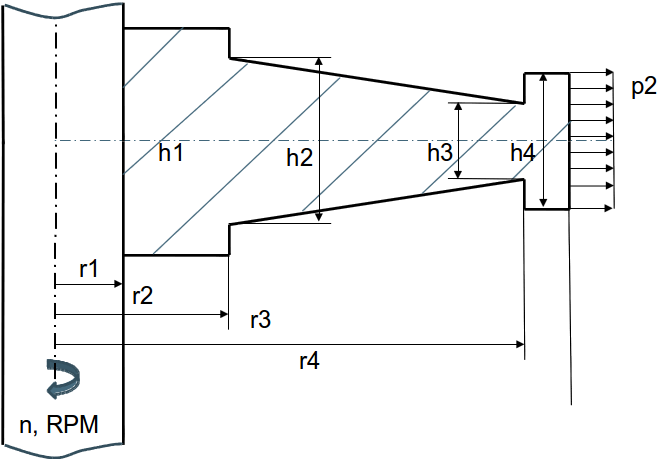
\includegraphics[width=0.4\textwidth]{figures/gp_on_grid/rotating_disk_parametrization.png}
  \caption{Rotating disc parametrization.}
  \label{fig:rotating_disc_parametrization}
\end{figure}

\begin{figure}
  \centering
  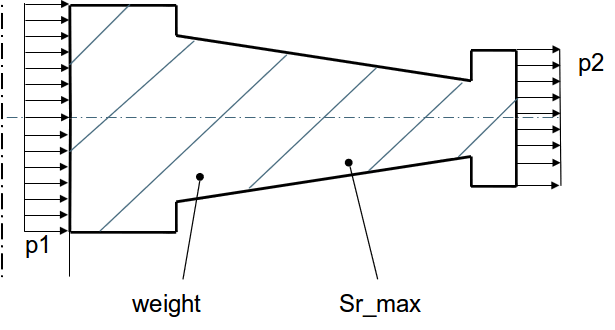
\includegraphics[width=0.4\textwidth]{figures/gp_on_grid/rotating_disk_objectives.png}
  \caption{Rotating disc objectives.}
  \label{fig:rotating_disc_objectives}
\end{figure}

It is a common practice to build approximations of objective functions in order to analyze them
and perform optimization \citep{forrester2008surrogateModelling}.
So, we applied the tensorGP-reg algorithm and FITC developed in this work to this problem.
The DoE was full factorial; the number of points in each dimension was $[1, 8, 8, 3, 15, 5]$, i.e.,
$x_1$ was fixed.
The number of points in factors differs significantly and the generated data set is anisotropic.
The overall number of points in the training sample was 14 400.

Figures \ref{fig:rotating_disc_originalGP} and \ref{fig:rotating_disc_tensorGP} depict 2D slices of contact pressure
approximations along $x_5, x_6$ variables.
As you can see, FITC model degenerates while tensorGP-reg provides a smooth and accurate approximation.

\begin{figure}
  \centering
  \begin{subfigure}[b]{0.45\textwidth}
      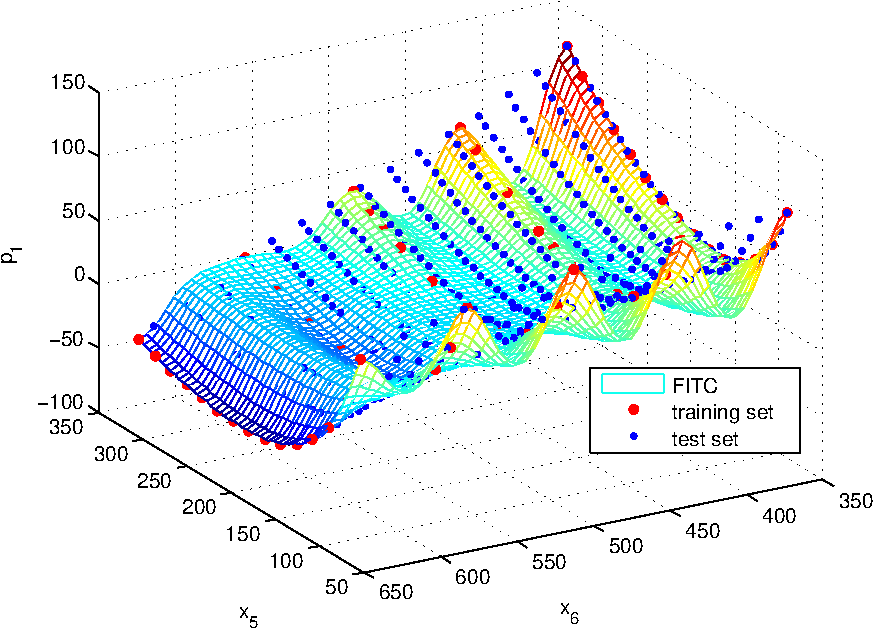
\includegraphics[width=\textwidth]{figures/gp_on_grid/rotating_disk_fitc.pdf}
      \caption{FITC.}
      \label{fig:rotating_disc_originalGP}
  \end{subfigure}
  \begin{subfigure}[b]{0.45\textwidth}
      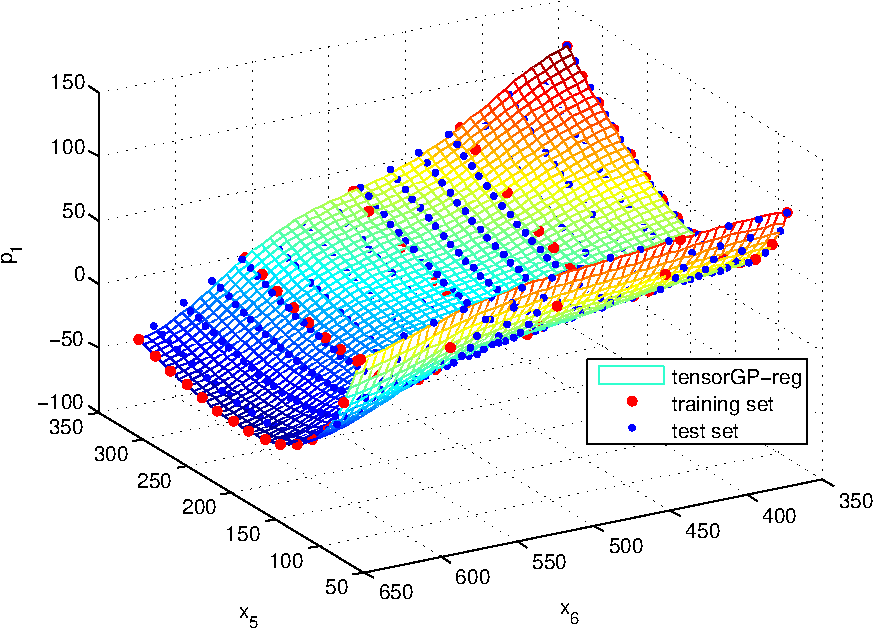
\includegraphics[width=\textwidth]{figures/gp_on_grid/rotating_disk_tensorGP.pdf}
      \caption{The proposed approach.}
      \label{fig:rotating_disc_tensorGP}
  \end{subfigure}
  \caption{2D slice along $x_5$ and $x_6$ variables (other variables are fixed) of tensorGP-reg approximation.}
\end{figure}

\section{Incomplete Factorial Design of Experiments}

A subset $\boldsymbol{\widetilde{\Omega}} \subseteq \boldsymbol{\Omega}$ of size
$\widetilde{N}$ of the full factorial DoE
is referred to as {\em incomplete factorial design of experiments}.
In general, taking a subset of $\Omega$ breaks the structure of the dataset,
so we cannot apply the same techniques described in the previous section.
However, the partial structure that is preserved can be of use,
though at a higher computational cost.
We use the same notation for the training set in this section
$\mathcal{D} = \{(\mathbf{x}_i, y_i)\}_{i=1}^{\widetilde{N}}$.

\subsection{Log-likelihood and posterior distribution calculation}

To calculate the log-likelihood and the posterior mean, we need to calculate
$\mathbf{K}_y^{-1}\mathbf{y}$ and the determinant $|\mathbf{K}_y|$.

Let $\mathbf{W}$ be a diagonal matrix of size $N \times N$,
where $N$ is the size of the full factorial DoE
$\boldsymbol{\widetilde{\Omega}} \supseteq \boldsymbol{\Omega}$.
Denote $R = N - \widetilde{N}$.
Let
$\mathbf{X} =
\{\mathbf{x}_i: \mathbf{x}_i \in \boldsymbol{\Omega}\}_{i = 1}^{N}$.
Then
\begin{equation*}
\mathbf{W}_{ii} =
\begin{cases}
    1, \mbox{ if } \mathbf{x}_i \in \boldsymbol{\Omega}, \\
    0, \mbox{ if } \mathbf{x}_i \notin \boldsymbol{\Omega}.
\end{cases}
\end{equation*}
We construct the vector $\mathbf{\widetilde{y}}$ as follows:
if $\mathbf{x}_i \in \boldsymbol{\widetilde{\Omega}}$,
then $\mathbf{\widetilde{y}}_i$ is filled with elements from $\mathbf{y}$
corresponding to $\mathbf{x}_i$.
We fill the rest of the elements of $\mathbf{\widetilde{y}}$ arbitrarily.
Now the matrix $\mathbf{\widetilde{K}}$ is the covariance matrix between points from
the set $\boldsymbol{\Omega}$.
Let us consider the following system of equations
\begin{equation}
\label{eq:incomplete_inverse}
\left (\mathbf{W \widetilde{K}} + \sigma^2_{noise}\mathbf{I} \right )\mathbf{z} =
\mathbf{W\widetilde{y}}.
\end{equation}
Notice that equations that correspond to missing values
have the form $\sigma_{noise}^2 \mathbf{z}_j = 0$.
Therefore, the elements of $\mathbf{z}$ that correspond to missing values are equal to zero.
The other elements are solutions of the equation $\mathbf{K}_y \mathbf{z}' = \mathbf{y}$,
which gives us $\mathbf{K}_y^{-1}\mathbf{y}$.
To solve \eqref{eq:incomplete_inverse}, we use conjugate gradients (CG) approach.
For CG, the matrix should be symmetric, so let's multiply the left hand side and the right hand
side by
$\mathbf{\widetilde{K}}$:
\[
\left (\mathbf{\widetilde{K} W \widetilde{K}} + \sigma^2_{noise}\mathbf{\widetilde{K}} \right) \mathbf{z} =
\mathbf{\widetilde{K}}\mathbf{W\widetilde{y}}.
\]
By substituting $\mathbf{\widetilde{z}} = \mathbf{\sqrt{K} z}$ we obtain
a system with lower condition number:
\[
\left (\mathbf{\sqrt{\widetilde{K}} W \sqrt{\widetilde{K}}} + \sigma^2_{noise} \mathbf{I} \right )\mathbf{\widetilde{z}} =
\mathbf{\sqrt{\widetilde{K}} W \widetilde{y}},
\]
where $\mathbf{\sqrt{\widetilde{K}}} = \mathbf{U \sqrt{D} U}^T$, $\mathbf{U}$ --- is a
matrix of eigenvectors of
$\mathbf{\widetilde{K}}$,
$\mathbf{D}$ --- is a diagonal matrix with eigenvalues of $\mathbf{\widetilde{K}}$.
Note that fast matrix-vector products can be calculated using the results of
the section \ref{sec:calc_loglikelihood}.

It is well known that CG converges at most in $r$ iterations, where
$r$ is a number of different eigenvalues of the system matrix \cite{nocedal2006numerical}.
In the system that we obtained, we can do such changes of variables,
so that the number of different eigenvalues is equal to either $R + 1$ or $\widetilde{N} + 1$:
\begin{enumerate}
\item Change of variables 1:
\[
\mathbf{z}_1 = \sqrt{\mathbf{\widehat{D}}} \mathbf{U}^T \mathbf{\widetilde{z}},
\]
where $\mathbf{\widehat{D}} = \mathbf{D} + \sigma^2_{noise}\mathbf{I}$.
The system of equations in this case looks like
\begin{equation}
\label{eq:variables_change_1}
        \left ( \sqrt{\mathbf{\widehat{D}}^{-1} \mathbf{D}} \mathbf{U}^T (\mathbf{W - I})
            \mathbf{U}\sqrt{\mathbf{D \widehat{D}}^{-1}} + \mathbf{I}
        \right ) \mathbf{z}_1 = \sqrt{\mathbf{\widehat{D}}^{-1} \mathbf{D}} \mathbf{U}^T \mathbf{W \widetilde{y}}.
\end{equation}
\item Change of variables 2:
\[
\mathbf{z}_2 = \mathbf{U}^T \mathbf{\widetilde{z}}.
\]
In this case we obtain,
\begin{equation}
\label{eq:variables_change_2}
        \left ( \sqrt{\mathbf{D}} \mathbf{U}^T \mathbf{W}
            \mathbf{U}\sqrt{\mathbf{D}} + \sigma^2_{noise}\mathbf{I}
        \right ) \mathbf{z}_2 = \sqrt{\mathbf{D}} \mathbf{U}^T \mathbf{W \widetilde{y}}.
\end{equation}
\end{enumerate}

\begin{proposition}
The matrix of the system of equations \eqref{eq:variables_change_1} has no more than $R + 1$
different eigenvalues,
while the matrix \eqref{eq:variables_change_2} has no more than $\widetilde{N} + 1$.
\end{proposition}
\begin{proof}
    Let us show the proof for \eqref{eq:variables_change_2}.
    The statement for \eqref{eq:variables_change_1} can be proved similarly.
    The rank of matrix $\mathbf{W}$ is equal to $\widetilde{N}$.
    As the rank of the product of matrices is not greater than the rank of the factors,
    the rank of the matrix
    $\mathbf{A} = \sqrt{\mathbf{D}} \mathbf{U}^T \mathbf{W} \mathbf{U}\sqrt{\mathbf{D}}$
    is not greater than $\widetilde{N}$.
    Now, the matrix $\mathbf{A}$ is symmetric and has $N$ real eigenvalues
    $\lambda_i, i = 1, \ldots, N$.
    Moreover, as the rank is not greater than $\widetilde{N}$, the number of different eigenvalues
    is not greater than $\widetilde{N}$ either.
    The eigenvalues of the matrix in \eqref{eq:variables_change_2}
    are equal to $\lambda_i + \sigma^2_{noise}$.
    Hence, the matrix has no more than $\widetilde{N} + 1$ different eigenvalues.
\end{proof}


The computational complexity of one iteration of CG is the same as the complexity
of computing $\mathbf{\widetilde{K}}_y \mathbf{x}$,
therefore, the overall complexity of computing $\mathbf{K}_y^{-1}\mathbf{y}$ is
\[
\mathcal{O}\left (\min\{R + 1, \widetilde{N} + 1\} N\sum_{i = 1}^K n_i \right ).
\]
Assuming
that $n_i \ll N$ (i.e., the number of factors is large, and their sizes are equal),
we obtain
$\mathcal{O}(\min\{R + 1, \widetilde{N} + 1\} N^{1 + \frac{1}{K}})$.
So, if less than half of the points are missing, the complexity is linear in the number of missing points.
$\mathcal{O}((R + 1)N^{1 + \frac{1}{K}})$.
In the limit, when there are no missing points, the complexity is the same
as the complexity for full factorial DoE.


\subsection{Calculation of the determinant}
Let $\mathbf{A}$ be a covariance matrix of size $N \times R$ between training points and
missing points,
and $\mathbf{B}$ be a covariance matrix of size $R \times R$ between missing points.
Then matrix $\mathbf{\widetilde{K}}_y$ can be represented as a block matrix
\[
\mathbf{\widetilde{K}_y} = \begin{pmatrix}
  \mathbf{K}_y & \mathbf{A} \\
  \mathbf{A}^T & \mathbf{B}
\end{pmatrix}.
\]
The determinant of the block matrix can be calculated as follows
$|\mathbf{\widetilde{K}}_y | = |\mathbf{K}_y| |\mathbf{B} - \mathbf{A}^T \mathbf{K}_y^{-1}\mathbf{A}|$,
therefore, the determinant of interest is given by
\begin{equation}
\label{eq:determinant_incomplete}
|\mathbf{K}_y| = \frac{|\mathbf{\widetilde{K}}_y |}{|\mathbf{B} - \mathbf{A}^T \mathbf{K}_y^{-1}\mathbf{A}|}.
\end{equation}
The computational complexity of this expression is
$\mathcal{O}(\min\{R + 1, \widetilde{N} + 1\} R N\sum_{i = 1}^K n_i)$,
because we need to calculate matrix-vector multiplication $\mathbf{K}_y^{-1}\mathbf{A}_i$
$R$ times,
where $\mathbf{A}_i$ is an $i$-th column of matrix $\mathbf{A}$.
The memory complexity equals $\mathcal{O}(R\widetilde{N} + N + \sum_{i = 1}^K n_i^2)$.

However, we can reduce memory to $\mathcal{O}(\widetilde{N})$ and improve the constant in the complexity of
\eqref{eq:determinant_incomplete}.
For this, notice that the approach to calculate $\mathbf{K}_y^{-1}\mathbf{y}$
also allows to calculate $\mathbf{C}^{-1}\mathbf{v}$,
where $\mathbf{C}$ is an arbitrary principal submatrix of size $m \times m$
of the matrix $\mathbf{\widetilde{K}}_y$,
and $\mathbf{v}$ is any vector of length $m$.
The computational complexity of the operation in this case is
$\mathcal{O} \left (\min\{m + 1, \widetilde{N} - m + 1\}
\widetilde{N}\sum_{i = 1}^K n_i \right )$.

Denote
\[
\mathbf{\widetilde{K}}_y = \begin{pmatrix}
  \mathbf{K}_1 & \mathbf{a}_1 \\
  \mathbf{a}_1^T & b_1
\end{pmatrix},
\]
where $\mathbf{K}_1$ is of size $(\widetilde{N} - 1) \times (\widetilde{N} - 1)$,
$\mathbf{a}_1$ is a vector of length $\widetilde{N} - 1$, $b_1$ is a scalar.
Then
\[
|\mathbf{\widetilde{K}}_y| = |\mathbf{K}_1| (b_1 - \mathbf{a}_1^T \mathbf{K}_1^{-1}\mathbf{a}_1).
\]
Similarly, splitting $\mathbf{K}_1$ into blocks
$\begin{pmatrix}
\mathbf{K}_2 & \mathbf{a}_2 \\
\mathbf{a}_2 & b_2
\end{pmatrix}$,
and splitting matrix $\mathbf{K}_2$ into
$\begin{pmatrix}
\mathbf{K}_3 & \mathbf{a}_3 \\
\mathbf{a}_3 & b_3
\end{pmatrix}$,
and so on, we obtain
\[
|\mathbf{\widetilde{K}}_y| =
|\mathbf{K}_y| \prod_{i = 1}^R(b_i - \mathbf{a}_i^T\mathbf{K}_i^{-1}\mathbf{a}_i),
\]
or
\begin{equation}
\label{eq:determinant_incomplete_practical}
|\mathbf{K}_y| =
\frac{|\mathbf{\widetilde{K}}_y|}{\prod_{i = 1}^R(b_i -
\mathbf{a}_i^T\mathbf{K}_i^{-1} \mathbf{a}_i)}.
\end{equation}
Here, to calculate the right hand side, we need to store only $\mathbf{K}_i^{-1}\mathbf{a}_i$,
therefore, the total memory complexity is $\mathcal{O}(N + \sum_{i = 1}^K n_i^2)$.

The complexity of the calculation of each $\mathbf{K}_i^{-1}\mathbf{a}_i$ is lower
than the complexity of the calculation of $\mathbf{K}_y^{-1}\mathbf{A}_i$,
thus, the expression \eqref{eq:determinant_incomplete_practical} is more efficient,
although asymptotically, it is the same.


\subsection{Experiments}
To compare the classical approach for GP regression against the proposed approach,
we generated several datasets with incomplete factorial DoE.
The dimensionality of input is $5$, factor sizes are equal to $[5, 4, 4, 4, 4]$, the number of missing points varies from $100$ to $320$.
In \fig{time_itgp}, you can see the ratio of the computation time of the standard approach (GP)
and the training time of the proposed approach (iTensorGP) for different number of missing
values.
Theory shows that the ratio should be $\frac{(N - R)^3}{R^2 N(\sum_{i = 1}^K n_i)}$.
Then the number of missing points increases, and so does the training time of iTensorGP.
At some points, iTensorGP becomes less efficient than the standard GP approach.
However, in case of a small amount of missing points, iTensorGP is much faster.

\begin{figure}
  \centering
  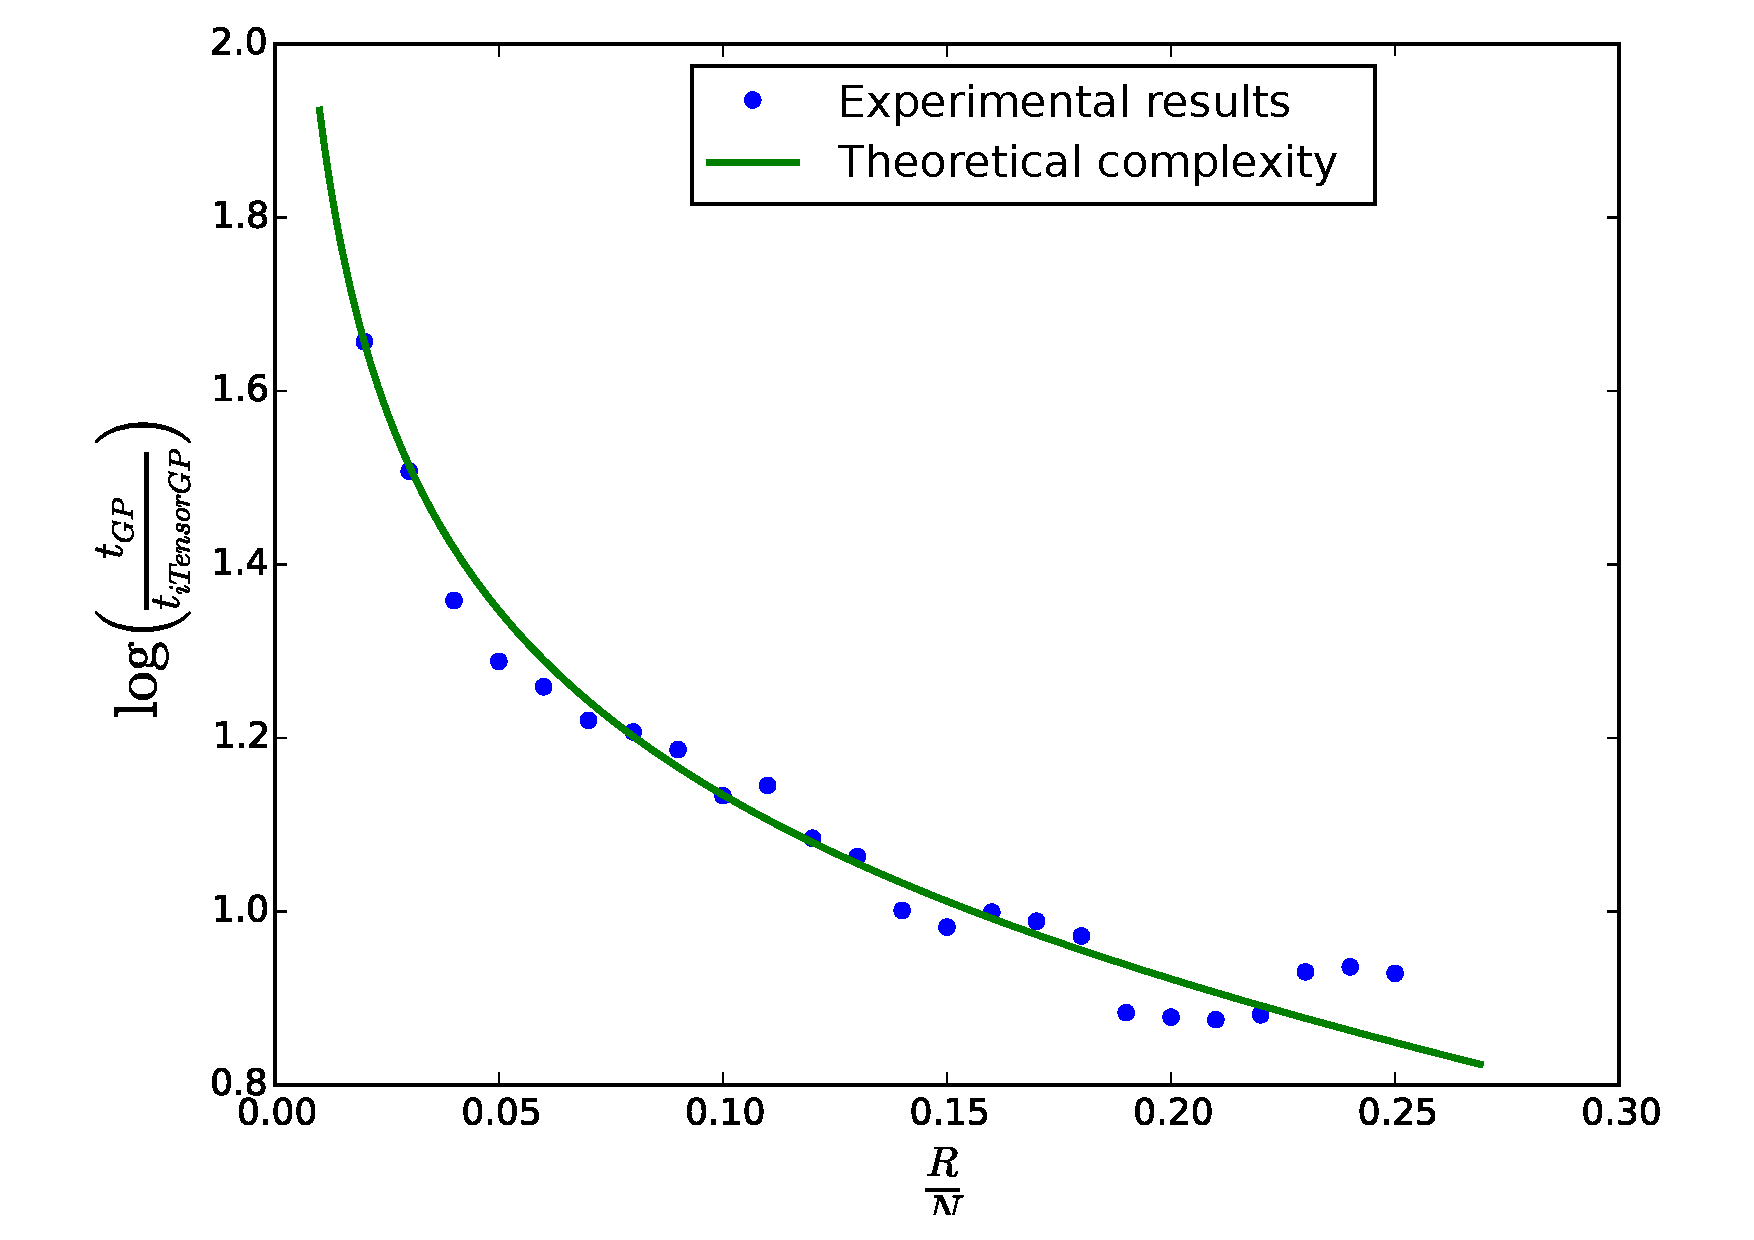
\includegraphics[width=0.5\textwidth]{figures/incomplete_grid/time_comparison_itgp.pdf}
  \caption{Comparison of the training time of the proposed approach (iTensorGP) and
  standard approach (GP).}
  \label{fig:time_itgp}
\end{figure}


